%\section{Background: On Model Typing} 
%
%- Model Typing to achieve substitutability, 
%- subtyping relation, 
%- class matching relation
%==> limitation : the class matching relation is not taken into account of the matching of the contracts.
%	
%%%%%%

\section{Background}\label{background}

In this section, we describe the concepts underlying our use of model types to support model substitutability.
%Model typing provides a well-defined theory that considers models as first-class entities, and typed by their respective model types~\cite{Steel07}, where model substitutability is achieved through subtyping relations between model types.  These relations enable a model typed by $A$ to be safely used where a model typed by $B$ is expected, $A$ and $B$ being model types.
We first present the MOF (Meta-Object Facility) meta-language, the basis for metamodels, and thus model manipulation operators. We then give an overview of model types as currently defined and implemented \cite{Steel07,ecmfa12}, and describe the limitations addressed by the approach presented in this paper. 

\subsection{Metamodeling}

{\em The Meta-Object Facility} (MOF)~\cite{MOF} is the OMG's standardized meta-language, i.e., a language to define metamodels. As such, it is a common basis for a vast majority of modeling languages and tools. A metamodel defines a set of models on which it is possible to apply common operators. The model substitutability approach presented in this paper is applicable to models expressed in languages with MOF metamodels. 

%\begin{figure}[tb]
%	\center
%	\includegraphics[scale=0.6]{fig/MOF.pdf}
%	\caption{The EMOF core with class diagram notation}
%	\label{MOF}
%\end{figure}

%Figure~\ref{MOF} displays the structure of EMOF (Essential MOF) which contains the core of the MOF meta-language in the form of a class diagram. E
MOF supports the definition of metamodels using \texttt{Classes} and \texttt{Properties}.\\ \texttt{Classes} can be abstract (i.e., they cannot be instantiated) and have \texttt{Properties} and \texttt{Operations}, which respectively declare attributes and references, and the signatures of methods available to the modeled concept. 
%\texttt{Classes} can have several super classes, from which they inherit all \texttt{Properties} and \texttt{Operations}.
A \texttt{Property} can be composite (an object can only be referenced through one composite \texttt{Property} at a given instant), derived (i.e., calculated from other \texttt{Properties}) and read-only (i.e., cannot be modified). A \texttt{Property} can also have an opposite \texttt{Property} with which it forms a bidirectional association.
%An \texttt{Operation} declares the \texttt{Types} of the exceptions it can raise and ordered \texttt{Parameters}.
%\texttt{Propertys}, \texttt{Operations}, and \texttt{Parameters} are \texttt{TypedElements}; their type can be either: a \texttt{Datatype} (\eg \texttt{Boolean}, \texttt{String}, etc.) or a \texttt{Class}.
%\texttt{Parameters}, \texttt{Properties} and \texttt{Operations} are \texttt{Multiplicity Elements}. As such, they have a multiplicity (defined by a lower and an upper bound), as well as orderedness and uniqueness.


{\em Metamodels} can be viewed as class diagrams in which each metamodel element can be instantiated to obtain objects representing model elements. However, metamodel elements are themeslves instances of MOF elements and thus a metamodel can be drawn as an object diagram where each concept is an instance of one of the MOF elements (e.g., \texttt{Class} or \texttt{Property} classes).

%Because model subtyping takes place at the metamodel level, the latter representation facilitates the definition of model subtyping relations by depicting metamodels and their contained concepts as objects with attributes and properties. 
%Thus, we will use the object diagram representation in preference to the more common class diagram one.

\subsection{Model Typing}\label{modeltyping}

{\em Model Types} were introduced by Steel \etal \cite{Steel07}, as an extension of object typing to provide abstractions about the object type level and enable the reuse of model manipulation operators.  Informally, a model type is a substructure (referred to as a {\em type group}) of the metamodel's class diagram.  It is important to distinguish the usage of the term metamodel from model type. We use the term metamodel to refer to the class diagram used to define a language, and when the same class diagram is used to define the type of a model it is called an {\em exact type}. It is also important to note that a model has one and only one metamodel to which it must conform, but the same model can have several model types, where each model type is a substructure of the metamodel. Because model types and metamodels share the same structure, it is possible to extract the exact type of a model from its metamodel. Figure~\ref{3lvl} represents a model $m_1$ that conforms to a metamodel $MM_1$ and is typed by model types $MT_A$ and $MT_B$, where $MT_B$ is the \emph{exact type} of $m_1$ that is extracted from $MM_1$. Both metamodels and model types conform to MOF.
\begin{figure}[tb]
	\center
	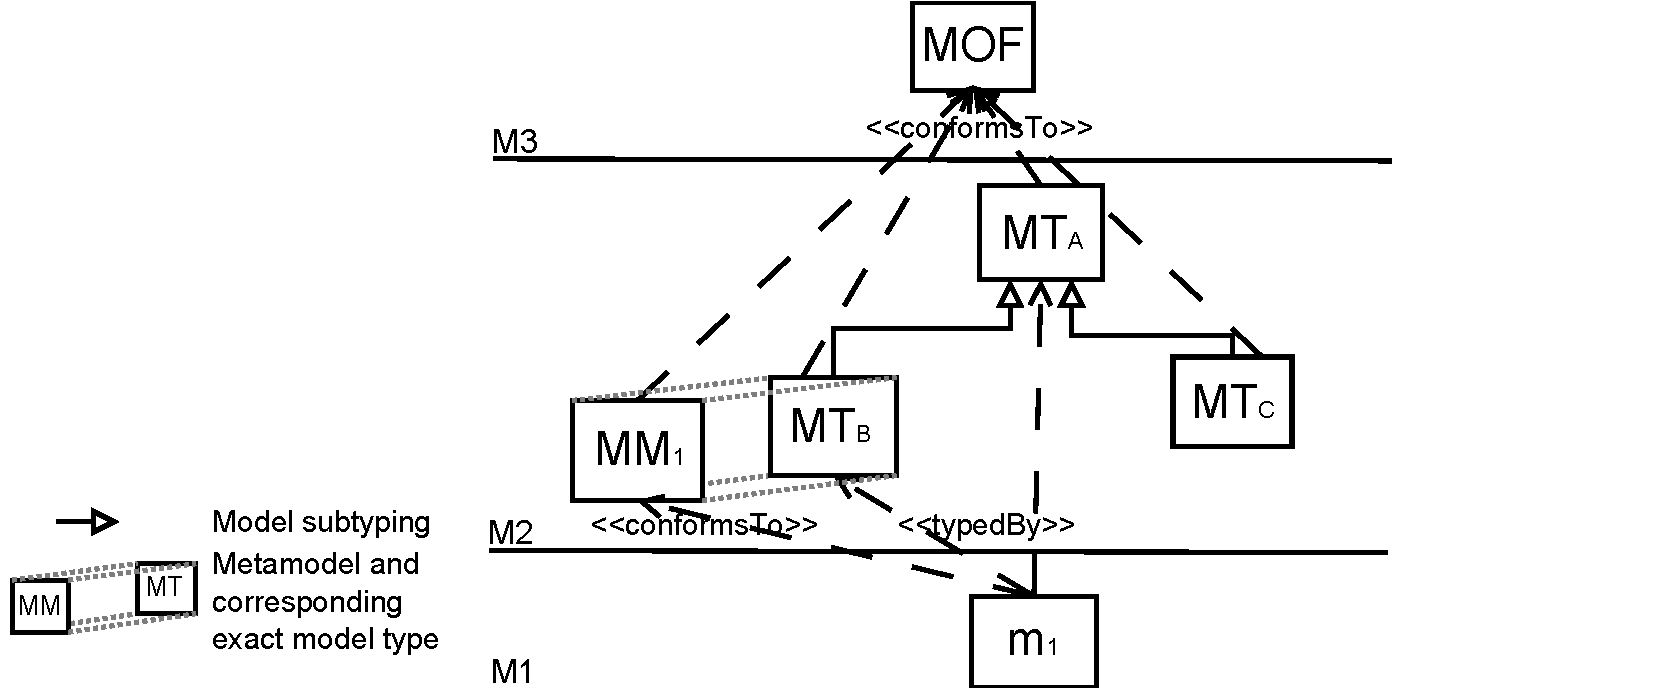
\includegraphics[scale=0.37]{fig/3levels2.pdf}
	\caption{Conformance, model typing and model subtyping relations}
	\label{3lvl}
\end{figure}
Given the above, a model type can be defined as follows:
\begin{definition}\label{modeltypedef}
\deftitle{Model type}
A model type is a substructure of a metamodel's class structure. A model does not have to include instantiations of each class in an associated model type, that is, the set of classes of elements in a model can be smaller than the classes in its model type.
\end{definition}

{\em Substitutability} is the ability to safely use an object of type $A$ where an object of type $B$ is expected. 
Substitutability is supported through subtyping in object-oriented languages. However, object subtyping does not handle specializations of model substructures (or {\em type groups})\footnote{For further information on type groups see Ernst's paper~\cite{Ernst01}.}. 
%Such type group specialization have been explored by K\"{u}hne in the context of MDE~\cite{Kuhne12}. K\"{u}hne defines three model specialization relations (specification import, conceptual containment and subtyping) implying different level of compatibility. We are only interested here in the third one, subtyping, which requires an \emph{uncompromised mutator forward-compatibility}, \eg substitutability, between instances of model types.
%\subsubsection{MOF Class Matching}
One way to safely reuse a model manipulation operation created for a model typed by $MT_A$ on a model typed by $MT_B$ is to ensure that $MT_A$ contains elements that can be substituted by elements defined by $MT_B$. 
%Since only model types conforming to MOF are currently considered, this can be done by ensuring the MOF elements from $MT_B$ (\eg classes, properties, operations) substitutable for those contained by $MT_A$. 
However, it is not possible to achieve model type substitutability through object subtyping. Thus, model typing uses an extended definition of \emph{object type matching} introduced by Bruce \etal \cite{Bruce03}, namely \emph{MOF Class Matching}.

\begin{definition}
\deftitle{MOF class matching}
MOF class $T'$ matches $T$ (written $T' \match T$) iff their names are equal, and for each property (respectively method) in $T$ there is a corresponding property (respectively method) in $T'$.
\end{definition}

The \emph{MOF class matching} relation can be seen as a kind of \emph{object type matching} relation that is tailored to MOF concepts.
Based on the \emph{MOF class matching} relation, we can achieve model type substitutability by defining a subtyping relation as follows:

\begin{definition}
\deftitle{Subtyping relationship for model types}
The model type \emph{subtyping} relation is a binary relation $\sqsubseteq$ on $ModelType$, the set of all model types, such that $(MT_B, MT_A) \in \sqsubseteq$ (also written $MT_B \sqsubseteq MT_A$) iff  $\forall$ $T_A$ $\in$ $MT_A$, $\exists$ $T_B$ $\in$ $MT_B$ such that $T_B$ $\match$ $T_A$.
\end{definition}

We recently introduced four extended subtyping relations between model types that take into account two additional criteria: The presence of heterogeneities between two model types (using adaptation) and the considered subset of the model types (using model type pruning) \cite{ecmfa12}.

%\subsubsection{Limits of Model Subtyping}
The \emph{subtyping} relation as currently defined has shortcomings. 
In particular, the current model typing definition and implementation only considers MOF-based metamodels as model types (through the \emph{MOF class matching} relation). Unfortunately, MOF delegates the definitions of contracts (\eg pre and post-conditions or invariants) to other languages (\eg OCL, the Object Constraint Language~\cite{OCL}). 
%Hence neither the original paper on model typing~\cite{Steel07} nor the follow-up \cite{ecmfa12} considers contracts in subtyping relations, but focuses on features of object types contained by model types. 
This limits the applicability of model typing for safely reusing model manipulations where OCL contracts are needed to precisely specify the applicability of the model transformation or the structure on which the model transformation can be applied (see motivating examples in Section \ref{examples}). The approach described in this paper addresses this limitation.
